Proteins fulfil the fundamental processes of life. 
Proteins consist of amino acids,
the building blocks that link together into a linear sequence, 
as beads of a pearl necklace.
This linear sequence is called the primary structure. 
Local and distant interactions between amino acids in the sequence will determine the fold and biophysical properties, 
and thus the function of the protein (Fig. \ref{fig:local_distant}).
To understand the difference between local and distant interactions,
we can visualise this  with the pearl necklace metaphor.
Imagine yourself unhooking the necklace and placing both ends far away from each other, forming a straight line.
Which beads are close to each other? 
Each bead is closest to its directly connected neighbours, 
a bit farther to the neighbours of the neighbours,
even further to their neighbours, and so on...
By placing the necklace as a straight line,
we have essentially reduced a three-dimensional necklace to a one-dimensional sequence.
When speaking about local interaction, 
it is meant as interactions between between beads that are close to each other in this one-dimensional space.
Proteins are not straight lines of amino acids however.
Just as a pearl necklace can make curves and fold upon itself, 
so do proteins.
This way beads that are very far away from each other in sequence,
can be close to each other in three-dimensional space and form interactions.
These are called distant interactions.
Each protein has its own unique local and distant interactions.
This way, 
they fold into different shapes and can so specialise for specific tasks.

~\begin{figure}[h!]
	\centering
	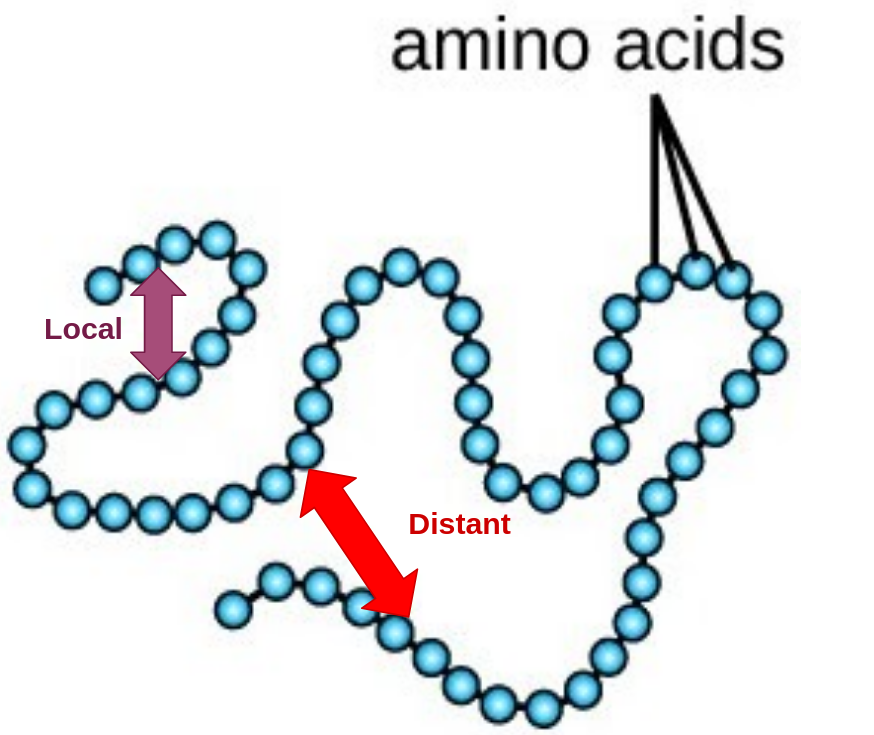
\includegraphics[width=0.6\linewidth]{./literature_review/proteins/img/local_distant.png}
	\caption{
		\textbf{Local and Distant interactions along the protein sequence}
		(adapted from https://tinyurl.com/y7aoehrt).
	}
	\label{fig:local_distant}
~\end{figure}
